% Options for packages loaded elsewhere
\PassOptionsToPackage{unicode}{hyperref}
\PassOptionsToPackage{hyphens}{url}
%
\documentclass[
]{book}
\usepackage{amsmath,amssymb}
\usepackage{lmodern}
\usepackage{ifxetex,ifluatex}
\ifnum 0\ifxetex 1\fi\ifluatex 1\fi=0 % if pdftex
  \usepackage[T1]{fontenc}
  \usepackage[utf8]{inputenc}
  \usepackage{textcomp} % provide euro and other symbols
\else % if luatex or xetex
  \usepackage{unicode-math}
  \defaultfontfeatures{Scale=MatchLowercase}
  \defaultfontfeatures[\rmfamily]{Ligatures=TeX,Scale=1}
\fi
% Use upquote if available, for straight quotes in verbatim environments
\IfFileExists{upquote.sty}{\usepackage{upquote}}{}
\IfFileExists{microtype.sty}{% use microtype if available
  \usepackage[]{microtype}
  \UseMicrotypeSet[protrusion]{basicmath} % disable protrusion for tt fonts
}{}
\makeatletter
\@ifundefined{KOMAClassName}{% if non-KOMA class
  \IfFileExists{parskip.sty}{%
    \usepackage{parskip}
  }{% else
    \setlength{\parindent}{0pt}
    \setlength{\parskip}{6pt plus 2pt minus 1pt}}
}{% if KOMA class
  \KOMAoptions{parskip=half}}
\makeatother
\usepackage{xcolor}
\IfFileExists{xurl.sty}{\usepackage{xurl}}{} % add URL line breaks if available
\IfFileExists{bookmark.sty}{\usepackage{bookmark}}{\usepackage{hyperref}}
\hypersetup{
  pdftitle={``Deployando'' Bookdown: un flujo de trabajo como modelo de edición digital ramificada, basada en estructuras descentralizadas, software libre y código abierto},
  pdfauthor={Andrés Lemos},
  hidelinks,
  pdfcreator={LaTeX via pandoc}}
\urlstyle{same} % disable monospaced font for URLs
\usepackage{longtable,booktabs,array}
\usepackage{calc} % for calculating minipage widths
% Correct order of tables after \paragraph or \subparagraph
\usepackage{etoolbox}
\makeatletter
\patchcmd\longtable{\par}{\if@noskipsec\mbox{}\fi\par}{}{}
\makeatother
% Allow footnotes in longtable head/foot
\IfFileExists{footnotehyper.sty}{\usepackage{footnotehyper}}{\usepackage{footnote}}
\makesavenoteenv{longtable}
\usepackage{graphicx}
\makeatletter
\def\maxwidth{\ifdim\Gin@nat@width>\linewidth\linewidth\else\Gin@nat@width\fi}
\def\maxheight{\ifdim\Gin@nat@height>\textheight\textheight\else\Gin@nat@height\fi}
\makeatother
% Scale images if necessary, so that they will not overflow the page
% margins by default, and it is still possible to overwrite the defaults
% using explicit options in \includegraphics[width, height, ...]{}
\setkeys{Gin}{width=\maxwidth,height=\maxheight,keepaspectratio}
% Set default figure placement to htbp
\makeatletter
\def\fps@figure{htbp}
\makeatother
\setlength{\emergencystretch}{3em} % prevent overfull lines
\providecommand{\tightlist}{%
  \setlength{\itemsep}{0pt}\setlength{\parskip}{0pt}}
\setcounter{secnumdepth}{5}
\usepackage{booktabs}
\ifluatex
  \usepackage{selnolig}  % disable illegal ligatures
\fi
\usepackage[]{natbib}
\bibliographystyle{apalike}

\title{``Deployando'' Bookdown: un flujo de trabajo como modelo de edición digital ramificada, basada en estructuras descentralizadas, software libre y código abierto}
\author{Andrés Lemos}
\date{2022-01-24}

\begin{document}
\maketitle

{
\setcounter{tocdepth}{1}
\tableofcontents
}
\hypertarget{portada}{%
\chapter*{Portada}\label{portada}}
\addcontentsline{toc}{chapter}{Portada}

\hypertarget{licencia-de-producciuxf3n-de-pares-versiuxf3n-legible-por-humanes}{%
\chapter*{Licencia de Producción de Pares (Versión legible por humanes)}\label{licencia-de-producciuxf3n-de-pares-versiuxf3n-legible-por-humanes}}
\addcontentsline{toc}{chapter}{Licencia de Producción de Pares (Versión legible por humanes)}

\begin{quote}
Esto es un resumen legible por humanos del \href{http://endefensadelsl.org/ppl_es.html}{texto legal (la licencia
completa)}
\#\# Ud. es libre de \{-\}
\end{quote}

\begin{itemize}
\tightlist
\item
  Compartir - copiar, distribuir, ejecutar y comunicar públicamente la obra
\item
  Hacer obras derivadas
\end{itemize}

\hypertarget{bajo-las-condiciones-siguientes}{%
\section*{Bajo las condiciones siguientes:}\label{bajo-las-condiciones-siguientes}}
\addcontentsline{toc}{section}{Bajo las condiciones siguientes:}

\begin{figure}
\centering

\includegraphics{images/by.png}
\caption{\textbf{Atribución} - Debe reconocer los créditos de la obra de la manera
especificada por el autor o el licenciante (pero no de una manera que sugiera
que tiene su apoyo o que apoyan el uso que hace de su obra).}
\end{figure}

\begin{figure}
\centering

\includegraphics{images/sa.png}
\caption{\textbf{Compartir bajo la Misma Licencia} - Si altera o transforma esta obra, o
genera una obra derivada, sólo puede distribuir la obra generada bajo una
licencia idéntica a ésta.}
\end{figure}

\begin{figure}
\centering

\includegraphics{images/nc.png}
\caption{\textbf{No Capitalista} - La explotación comercial de esta obra sólo está permitida
a cooperativas, organizaciones y colectivos sin fines de lucro, a
organizaciones de trabajadores autogestionados, y donde no existan relaciones
de explotación. Todo excedente o plusvalía obtenidos por el ejercicio de los
derechos concedidos por esta Licencia sobre la Obra deben ser distribuidos por y
entre los trabajadores.}
\end{figure}

\hypertarget{entendiendo-que}{%
\section*{Entendiendo que}\label{entendiendo-que}}
\addcontentsline{toc}{section}{Entendiendo que}

\begin{itemize}
\item
  \textbf{Renuncia} - Alguna de estas condiciones puede no aplicarse si se obtiene
  el permiso del titular de los derechos de autor.
\item
  \textbf{Dominio Público} - Cuando la obra o alguno de sus elementos se halle en
  el dominio público según la ley vigente aplicable, esta situación no quedará
  afectada por la licencia.
\item
  \textbf{Otros derechos} - Los derechos siguientes no quedan afectados por
  la licencia de ninguna manera:

  \begin{itemize}
  \item
    Los derechos derivados de usos legítimos u otras limitaciones
    reconocidas por ley no se ven afectados por lo anterior;
  \item
    Los derechos morales del autor;
  \item
    Derechos que pueden ostentar otras personas sobre la propia obra o
    su uso, como por ejemplo derechos de imagen o de privacidad.
  \end{itemize}
\item
  \textbf{Aviso} - Al reutilizar o distribuir la obra, tiene que dejar muy en cla
  los términos de la licencia de esta obra. La mejor forma de hacerlo es
  enlazar a esta página.
\end{itemize}

\hypertarget{intro}{%
\chapter{Introducción: Bookdown como herramienta de publicación ramificada}\label{intro}}

El flujo de trabajo que se propone a continuación, así como la composición, imposición y archivos digitales de este TPF, fueron realizados con herramientas de código abierto y de uso gratuito; principalmente Bookdown, GitHub y Zotero. El objetivo de este trabajo es explicar y documentar el desarrollo de un proyecto editorial que combina dichas herramientas en un flujo de trabajo basado en software libre y de acceso abierto, y que se orienta hacia un esquema de edición digital ramificada, descentralizada y distribuida.

Así, los métodos propuestos en este trabajo se organizan en un flujo editorial ramificado que consta de tres grandes etapas: componer, compilar y publicar (ver Figura \ref{fig:workflow} ). A grandes rasgos y a los efectos de este desarrollo, componer se refiere a producir los archivos fuente y darles formato en R \href{https://es.wikipedia.org/wiki/Markdown}{Markdown}, la versión del lenguaje de marcado Markdown optimizada para R; compilar consiste en aplicar un conjunto de comandos y fragmento de código de R para imponer y generar los archivos de salida; mientras que publicar consiste en la disposición pública de la publicación en alguna plataforma y/o soporte.

Es decir que, en el flujo de trabajo desarrollado, se combinan una forma particular de estructurar el proceso editorial a partir de la generación de un conjunto de archivos fuente y una metodología de concebir lo digital. Esta concepción apunta a que en un solo paso se generen múltiples publicaciones digitales para distintos propósitos, dispositivos y plataformas, a saber:

\begin{itemize}
\tightlist
\item
  Archivo del código fuente de la publicación en formato de extensión .md (Markdown) completo con rutas de acceso a imágenes estáticas para una fácil conversión a la plataforma del editor.
\item
  Edición web HMTL para el libro de acceso abierto, con iframes integrados a gráficos, videos, gifs y mapas interactivos.
\item
  Edición impuesta para imprenta, lectura digital en formato PDF enriquecido.
\item
  Edición en formato EPUB de acceso abierto, con iframes integrados a gráficos, videos, gifs y mapas interactivos.
\item
  Edición en formatos de extensión .doc (Microsoft Word) y .odt (Libreoffice) para obras derivadas, revisiones y comentarios.
\end{itemize}

Entonces, a diferencia de lo que ocurre en un flujo de trabajo editorial de tipo lineal, que requiere de la creación de archivos y códigos distintos para diferentes tipos de ediciones y publicaciones; en el esquema del flujo de trabajo ramificado, la producción de los originales, el seguimiento del proceso editorial, la revisión, la corrección, las colaboraciones y el control de cambios, ocurren todos sobre un mismo archivo y de forma paralela.



\begin{figure}

{\centering 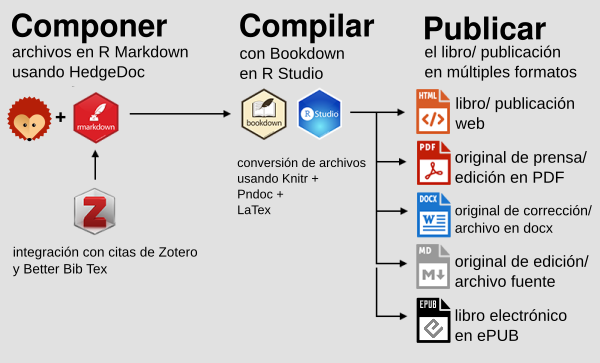
\includegraphics[width=0.8\linewidth]{images/workflow} 

}

\caption{Esquema simplificado de las etapas generales del flujo de trabajo, componer, compilar y publicar en múltiples formatos}\label{fig:workflow}
\end{figure}

\hypertarget{sobre-bookdown}{%
\section{Sobre Bookdown}\label{sobre-bookdown}}

El flujo de trabajo está desarrollado en \href{https://bookdown.org}{Bookdown}, un paquete de código abierto para el lenguaje de programación \href{https://www.r-project.org/}{R}, creado por Yihui Xie para la aplicación de escritorio gratuita \href{https://rstudio.com/}{RStudio}. Aunque mucha gente usa R para análisis estadístico, RStudio también es compatible con varias soluciones de publicación ramificada. Así, los pasos que forman parte de las tres grandes etapas (componer, compilar y publicar) de este flujo de trabajo estan determinadas por Bookdown:

\begin{enumerate}
\def\labelenumi{\arabic{enumi}.}
\tightlist
\item
  Durante la etapa de composición:
\end{enumerate}

\begin{itemize}
\item
  configuración de los archivos de Bookdown de forma que cada capítulo/ sección conste de un archivo de R Markdown (extensión .Rmd).
\item
  Organización de las citas, fuentes y referencias utilizando el administrador bibliográfico \href{https://zotero.org/}{Zotero} desarrollado por el \href{https://rrchnm.org/}{Centro Roy Rosenzweig de Historia y Nuevos Medios de la Universidad George Mason}. Además, hay que instalar la extensión Better \href{https://github.com/retorquere/zotero-better-bibtex}{BibTeX} para crear claves de citas en Zotero compatibles con Bookdown.
\end{itemize}

\begin{enumerate}
\def\labelenumi{\arabic{enumi}.}
\setcounter{enumi}{1}
\tightlist
\item
  Durante la etapa de compilación:
\end{enumerate}

\begin{itemize}
\item
  Creación de los archivos de salida utilizando el conversor universal de documentos \href{https://pandoc.org/}{PanDoc} y el software de preparación de documentos \href{https://www.latex-project.org/}{LaTeX}.
\item
  La capa de licenciamiento libre o abierto se puede configurar mediante una plantilla específica que se compile junto con el original. Esto se puede hacer incluso durante el proceso de escritura para hacer publicaciones parciales, generar capítulos promocionales, desarrollar la audiencia y hasta abrir la posibilidad de incorporar comentarios de lectorxs y colaboradores. Con las revisiones de cada jornada de trabajo se puede recompilar el libro, publicar las ediciones en el repositorio público de GitHub y usar el \href{https://pages.github.com/}{generador de sitios estáticos integrado} para alojar el formato web HTML de la publicación (libro/ publicación web).
\end{itemize}

\begin{enumerate}
\def\labelenumi{\arabic{enumi}.}
\setcounter{enumi}{2}
\tightlist
\item
  Durante la etapa de publicación:
\end{enumerate}

\begin{itemize}
\item
  Subida de los archivos fuente a un repositorio de \href{https://github.com/}{GitHub} (repo), que además de hacer posible la disposición pública de la publicación en internet mediante un sitio web; permite al equipo editorial, conocer las versiones del texto que se generan (traducción, corrección, revisión, ramificación, reedición, erc), planificar el proyecto, seguir el desarrollo del proceso editorial y los autores, trabajar simultáneamente en el libro/ publicación en un repositorio común.
\item
  Aplicar el modelo de \href{https://docs.microsoft.com/es-es/devops/deliver/what-is-infrastructure-as-code}{infraestructura como código} para alojar el libro/ publicación web gratuitamente mediante GitHub pages. De esta forma, el sitio web que se genera, no solamente funciona como un producto editorial en sí, sino que además puede funcionar como interfaz de acceso al resto de las versiones de la publicación o ediciones (pdf, epub, mobi ,docx y md).
\end{itemize}

Sin embargo, la descripción del flujo de trabajo desarrollado en Bookdown que se hace aquí, no es exhaustiva y comprende solo un conjunto de elementos de análisis pertinentes a los contenidos del Seminario de Publicaciones Digitales. Para obtener más detalles técnicos sobre Bookdown y ejemplos de otras publicaciones creadas con esta herramienta, se puede consultar \url{https://bookdown.org} \footnote{- Xie, Yihui. Bookdown: Authoring Books and Technical Documents with R Markdown. Chapman \& Hall/CRC, 2018. \url{https://bookdown.org/yihui/bookdown/}. - Xie, Yihui, J. J. Allaire, and Garrett Grolemund. R Markdown: The Definitive Guide. Chapman \& Hall/CRC, 2020. \url{https://bookdown.org/yihui/rmarkdown/}. - Xie, Yihui, Christophe Dervieux, and Emily Riederer. R Markdown Cookbook. Chapman \& Hall/CRC, 2020. \url{https://bookdown.org/yihui/rmarkdown-cookbook/}.}.

\begin{itemize}
\item
  Xie, Yihui. Bookdown: Authoring Books and Technical Documents with R Markdown. Chapman \& Hall/CRC, 2018. \url{https://bookdown.org/yihui/bookdown/}.
\item
  Xie, Yihui, J. J. Allaire, and Garrett Grolemund. R Markdown: The Definitive Guide. Chapman \& Hall/CRC, 2020. \url{https://bookdown.org/yihui/rmarkdown/}.
\item
  Xie, Yihui, Christophe Dervieux, and Emily Riederer. R Markdown Cookbook. Chapman \& Hall/CRC, 2020. \url{https://bookdown.org/yihui/rmarkdown-cookbook/}.
\end{itemize}

\hypertarget{cuxf3mo-instalar-y-configurar-bookdown}{%
\section{Cómo instalar y configurar Bookdown}\label{cuxf3mo-instalar-y-configurar-bookdown}}

A continuación, se enumeran los pasos que hay que seguir para configurar la plataforma de publicación (Bookdown) y las herramientas relacionadas necesarias para compilar este trabajo, utilizando Ubuntu 20.04. Esto no requiere conocimientos especiales sobre Linux, de forma que los pasos para la instalación y la configuración en Ubuntu, si bien son diferentes, son similares a los que se deben seguir para Windows y MacOs.

\begin{enumerate}
\def\labelenumi{\arabic{enumi}.}
\item
  Instalar el lenguaje de programación R \url{https://www.r-project.org}, requerido para usar Bookdown.
\item
  Instalar la versión gratuita de RStudio Desktop para facilitar el uso de R mediante la interfaz gráfica del editor de texto. Algunes autores componen sus textos directo en RStudio, pero es recomendable usar algún editor de texto (como \href{https://docutopia.tupale.co/}{HedgeDoc} ), ya que estos suelen tener comandos, atajos y opciones específicas que hacen más ágil la escritura.
\item
  Dentro de RStudio, dirigirse a la pestaña ``Packages'' y seleccionar ``Install'' ( \href{images/packages-install.png}{ver captura de pantalla} ).
\item
  Dentro de RStudio, instalar el paquete ``bookdown'' y seleccionar ``Install Dependencies'' ( \href{images/bookdown-install.png}{ver captura de pantalla} ).
\item
  Para que Bookdown cree la versión de la publicación en PDF hay que instalar un motor de \href{https://en.wikipedia.org/wiki/LaTeX}{LaTeX} que transforme los formatos de las citas e imágenes de Markdown a estilos de página preconfigurados. Dado que LaTeX es muy pesado, Bookdown recomienda el paquete TinyTeX que es más ligero. Para instalarlo, dentro de RStudio hay que seleccionar la pestaña ``Packages'', seleccionar ``Install'' y tipear ``tinytex'' para buscar y cargar el paquete ( \href{images/tinytex-install.png}{ver captura de pantalla} ).
\item
  Para terminar de instalar tinytex hay que escribir tinytex :: install\_tinytex () en la consola de RStudio y presionar ``return''. ( \href{images/tinytex-finish.png}{ver captura de pantalla} )
\item
  Junto con la instalación de RStudio, hay que instalar Pandoc, el paquete que convierte archivos del formato Markdown a HMTL y otros formatos. Para confirmar la instalación de Pandoc y el número de versión hay que escribir rmarkdown :: pandoc\_version () en la consola de RStudio, y presionar ``return''. El número de la versión instalada debe ser 2.3.1 o superior. Para instalar una versión más reciente de Pandoc, que es muy recomendable, dirigirse a \url{https://pandoc.org}.
\end{enumerate}

\hypertarget{componer}{%
\chapter{Componer}\label{componer}}

\hypertarget{estructura-de-archivos-y-encabezados}{%
\section{Estructura de archivos y encabezados}\label{estructura-de-archivos-y-encabezados}}

En general, cada capítulo es un archivo .Rmd independiente. Esto implica que, en caso de editar el contenido de la publicación en simultáneo, les coautorxs tienen que trabajar en diferentes capítulos del libro y enviar regularmente \emph{commits} al repositorio. Una alternativa para evitar conflictos en el repositorio es trasladar el proceso de escritura a un editor de texto externo especializado en Markdown que tenga control de versiones, que sea colaborativo y multiplataforma, como HedgeDoc. Del mismo modo, es recomendable que solamente une miembrx del equipo compile regularmente el libro con Bookdown para evitar conflictos de combinación de código.

\hypertarget{methods}{%
\chapter{Methods}\label{methods}}

We describe our methods in this chapter.

\hypertarget{applications}{%
\chapter{Applications}\label{applications}}

Some \emph{significant} applications are demonstrated in this chapter.

\hypertarget{example-one}{%
\section{Example one}\label{example-one}}

\hypertarget{example-two}{%
\section{Example two}\label{example-two}}

\hypertarget{final-words}{%
\chapter{Final Words}\label{final-words}}

We have finished a nice book.

  \bibliography{book.bib,packages.bib}

\end{document}
